\documentclass{exam}
\usepackage{../commonheader}

\title{Midterm Study Party}
\date{July 7, 2017}

\begin{document}
\maketitle

\section{Control}
\begin{questions}
\question Implement \lstinline$sum_k_digits$ which takes in two integers, \lstinline$n$ and \lstinline$k$ and sums the rightmost \lstinline$k$ digits of \lstinline$n$. If \lstinline$k$ is greater than \lstinline$n$, sum up all of the digits. 

\ifprintanswers\else
\begin{lstlisting}
def sum_k_digits(n, k):
    """Returns the sum of the rightmost k digits of n.

    >>> sum_k_digits(11111, 3)
    3
    >>> sum_k_digits(12345, 2)
    9
    """
    total = ______________________________________
    
    while ________________________________________:
    
        total = ______________________________________
        
        n = __________________________________________
        
        k = __________________________________________
    	
    return ___________________________________________
\end{lstlisting}
\fi

\begin{solution}
\begin{lstlisting}
def sum_k_digits(n, k):
    """Returns the sum of the rightmost k digits of n.
    
    >>> sum_k_digits(11111, 3)
    3
    >>> sum_k_digits(12345, 2)
    9
    """
    total = 0
    while k > 0:
        total = total + (n % 10)
        n = n // 10
        k = k - 1
    return total
\end{lstlisting}
\end{solution}

\question Implement \lstinline$sum_k_digits$ again except using recursion instead of iteration.

\begin{solution}
\begin{lstlisting}
def sum_k_digits(n, k):
	""" Returns the sum of the rightmost k digits of n. Assume n has >= k digits.

    >>> sum_k_digits(11111, 3)
    3
    >>> sum_k_digits(12345, 2)
    9
	"""
	if k == 0:
	   return 0
	return n % 10 + sum_k_digits(n // 10, k - 1)
\end{lstlisting}
\end{solution}
\end{questions}
\clearpage

\section{Environment Diagrams}
\begin{questions}
\question Fill in the environment diagram that results from executing the code below until the entire program
is finished or an error occurs. You may not need to use all of the spaces or frames.

A complete answer will:
\begin{itemize}
\item Add all missing names and parent annotations to all local frames.
\item Add all missing values created or referenced during execution.
\item Show the return value for each local frame. 
\end{itemize}

\begin{lstlisting}
sam = "ss"

def josiah(leo):
    sam = "it"
    def josh(cj):
        donna = cj(sam, "sag") 
        return donna + leo
    return josh

president = josiah("tarius")
password = president(lambda josh, toby: toby + josh)
\end{lstlisting}

\begin{solution}
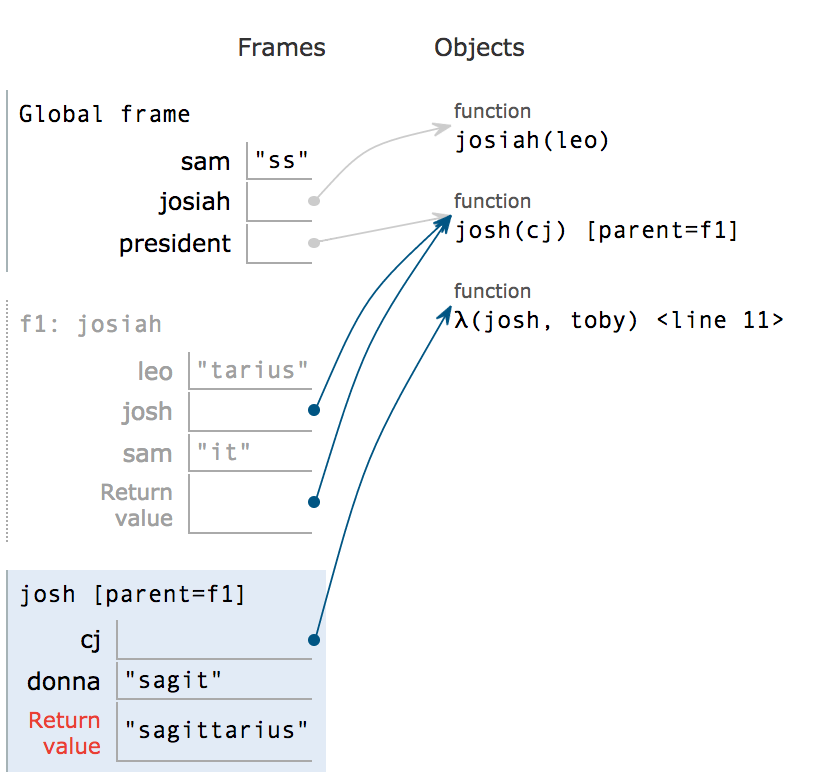
\includegraphics[width=7cm]{env1}
\end{solution}

\clearpage

% \question Fill in the environment diagram that results from executing the code below until the entire program
% is finished or an error occurs. You may not need to use all of the spaces or frames.
% 
% A complete answer will:
% \begin{itemize}
% \item  Add all missing names and parent annotations to all local frames.
% \item  Add all missing values created or referenced during execution.
% \item Show the return value for each local frame. 
% \end{itemize}
% 
% \begin{lstlisting}
% def never(the, less):
%     if the < less:
%         return 'never'
%     elif not less:
%         print('always')
%     if less == -3:
%         return never(less, the)
%     return never(less, less - the)
% 
% never(3, 0)
% \end{lstlisting}
% 
% \begin{solution}
% 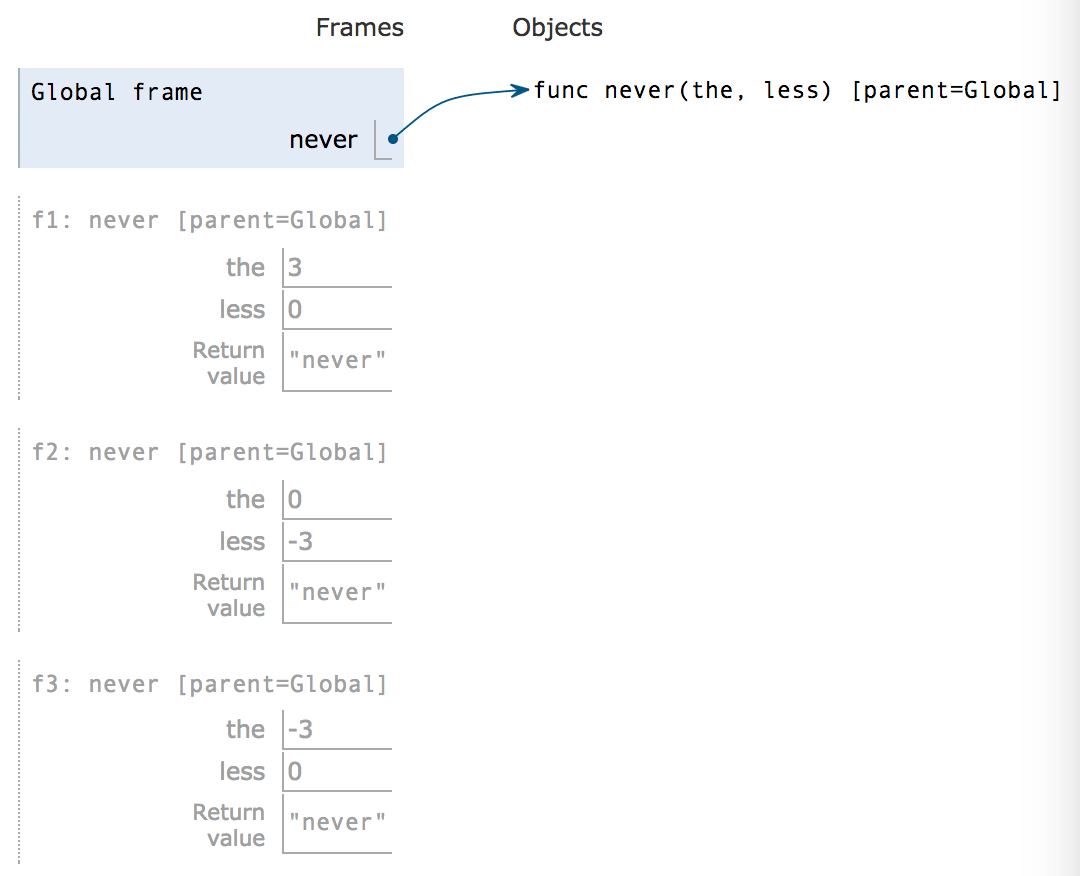
\includegraphics[width=10cm]{env2}
% \end{solution}
\end{questions}

\clearpage

\section{What Would Python Display?}
\begin{questions}
\question For each of the expressions in the table below, write the output displayed by the interactive Python interpreter when the expression is evaluated. The output may have multiple lines. If an error occurs, write ``Error''.

Assume that you have started \texttt{python3} and executed the following statements:

\begin{lstlisting}
def pup(bark):
    woof = 10
    def yip(yap):
        if bark % yap == 0:
            return woof * 3
        return yap + woof
    return yip

def spot(dog):
    per = 39
    if dog > 5:
        print("pup")
    if dog > 10:
        return pup(per)

def cloud(grr):
    print(grr * 3)

woof = 9
\end{lstlisting}
\vspace*{-0.25in}

\ifprintanswers\else
\begin{center}
\begin{tabular}{|m{8cm}|m{6cm}|}
\hline
\textbf{Expression} & \textbf{Interactive Output} \\
\hline
\lstinline$py = woof // 3$ & \\ [2em]
\hline
\lstinline$pet = spot(13)$ & \\ [3em]
\hline
\lstinline$print(cloud(woof + 6))$ & \\ [3em]
\hline
\lstinline$pet(py)$ & \\ [3em]
\hline
\lstinline$pet(woof)$ & \\ [3em]
\hline
\lstinline$pup(py)$ & \\ [3em]
\hline
\lstinline$pet(3)$ & \\ [3em]
\hline
\end{tabular}
\end{center}
\fi

\begin{solution}
\begin{center}
\begin{tabular}{|m{8cm}|m{6cm}|}
\hline
\textbf{Expression} & \textbf{Interactive Output} \\
\hline
\lstinline$py = woof // 3$ & \\ [2em]
\hline
\lstinline$pet = spot(13)$ & \color{red}\texttt{pup} \\ [3em]
\hline
\lstinline$print(cloud(woof + 6))$ & \color{red}\texttt{45} \\ \texttt{None} \\ [3em]
\hline
\lstinline$pet(py)$ & \color{red}\texttt{30} \\ [3em]
\hline
\lstinline$pet(woof)$& \color{red}\texttt{19} \\ [3em]
\hline
\lstinline$pup(py)$ & \color{red}\texttt{Function} \\ [3em]
\hline
\lstinline$pet(3)$ & \color{red}\texttt{30} \\ [3em]
\hline
\end{tabular}
\end{center}
\end{solution}

% \question For each of the expressions in the table below, write the output displayed by the interactive Python interpreter when the expression is evaluated. The output may have multiple lines. If an error occurs, write ``Error''.
% 
% Assume that you have started \texttt{python3} and executed the following statements:
% 
% \begin{lstlisting}
% def dell(ta):
%     lamduh = [3, 1, 4, 1, 5, 9]
%     pie = lamduh
%     def eye(ota):
%         return lambda pie, kye: pie[:-2] + kye[ota[0]::-1]
% 
%     lamduh = lamduh + ta
%     print(pie)
%     return eye
% 
% def bay(ta):
%     row = [ca - 9 for ca in ta]
%     print(row, ta)
%     return dell
% \end{lstlisting}
% 
% \ifprintanswers\else
% \begin{center}
% \begin{tabular}{|m{8cm}|m{6cm}|}
% \hline
% \textbf{Expression} & \textbf{Interactive Output} \\
% \hline
% \lstinline$fie = [2, 17, 20, 17]$ & \\ [2em]
% \hline
% \lstinline$nul = [0, -1, -50]$ & \\ [2em]
% \hline
% \lstinline$gam = bay(fie)$ & \\ [3em]
% \hline
% \lstinline$tao = gam(nul)$ & \\ [3em]
% \hline
% \lstinline$print(tao([1, 5, 7])(fie, nul))$ & \\ [3em]
% \hline
% \end{tabular}
% \end{center}
% \fi
% 
% \begin{solution}
% \begin{center}
% \begin{tabular}{|m{8cm}|m{6cm}|}
% \hline
% \textbf{Expression} & \textbf{Interactive Output} \\
% \hline
% \lstinline$fie = [2, 17, 20, 17]$ & \\ [2em]
% \hline
% \lstinline$nul = [0, -1, -50]$ & \\ [2em]
% \hline
% \lstinline$gam = bay(fie)$ & \color{red}\texttt{[-7, 8, 11, 8]} \\ \texttt{[2, 17, 20, 17]} \\ [3em]
% \hline
% \lstinline$tao = gam(nul)$ & \color{red}\texttt{[3, 1, 4, 1, 5, 9]} \\ [3em]
% \hline
% \lstinline$print(tao([1, 5, 7])(fie, nul))$& \color{red}\texttt{[2, 17, -1, 0]} \\ [3em]
% \hline
% \end{tabular}
% \end{center}
% \end{solution}
\end{questions}

\section{Lists}
\begin{questions}
\question What Would Python Display?

\ifprintanswers\else
\begin{lstlisting}
>>> x = [1, 2, 3, 4, 5]
>>> x[0]

>>> x[4]

>>> x[-1]

>>> x[1:]

>>> x[:5]

>>> x[::-1]

>>> x[::-2]

>>> x = [1, 2, 3, [4, 5]]
>>> y = [0] + x
>>> x, y
\end{lstlisting}
\fi

\begin{solution}
\begin{lstlisting}
>>> x = [1, 2, 3, 4, 5]
>>> x[0]
1
>>> x[4]
5
>>> x[-1] 
5
>>> x[1:]
[2, 3, 4, 5]
>>> x[:5]
[1, 2, 3, 4, 5]
>>> x[::-1]
[5, 4, 3, 2, 1]
>>> x[::-2]
[5, 3, 1]
>>> x = [1, 2, 3, [4, 5]]
>>> y = [0] + x
>>> x, y
[1, 2, 3, [4, 5]], [0, 1, 2, 3, [4, 5]]
\end{lstlisting}
\end{solution}

\clearpage

\question Mario needs to jump over a sequence of Piranha plants, represented as a string of dashes and P's. He only moves forward and can either step (move forward one space) or jump (move forward two spaces) from each position. How many different ways can Mario traverse a level without stepping or jumping into a Piranha plant? Assume that every level begins with a dash (where Mario starts) and ends with a dash (where Mario must end up):

\begin{lstlisting}
def mario_number(level):
    """
    >>> mario_number('-P-P-')   # jump, jump 
    1 
    >>> mario_number('-P-P--')  # jump, jump, step 
    1
     >>> mario_number('--P-P-') # step, jump, jump 
    1   
    >>> mario_number('---P-P-') # step, step, jump, jump; jump, jump, jump 
    2 
    >>> mario_number('-P-PP-')  # Mario cannot jump two plants 
    0 
    >>> mario_number('----')    # step, jump; jump, step; step, step, step
    3
    """
\end{lstlisting}

\begin{solution}
\begin{lstlisting}
    if len(level) == 0 or level[0] == 'P':
        return 0
    elif len(level) <= 2:
        return 1
    else:
        return mario_number(level[1:]) + mario_number(level[2:])
\end{lstlisting}
\end{solution}
\end{questions}

\clearpage

\section{Higher Order Functions}
\begin{questions}
\question Implement the \lstinline$memory$ function, which takes a number \lstinline$x$ and a single-argument function \lstinline$f$. It returns a function with a peculiar behavior that you must discover from the doctests. You may only use names and call expressions in your solution. You may not write numbers or use features of Python not yet covered in the course.

\begin{lstlisting}
square = lambda x: x * x
double = lambda x: 2 * x
\end{lstlisting}

\ifprintanswers\else
\begin{lstlisting}
def memory(x, f):
    """ Return a higher - order function that prints its memories.
    >>> f = memory (3 , lambda x: x)
    >>> f = f(square)
    3
    >>> f = f(double)
    9
    >>> f = f(print)
    6
    >>> f = f(square)
    3
    None
    """
    def g(h):

        print(_______________________________________________)

        return ______________________________________________

    return g
\end{lstlisting}
\fi

\begin{solution}
\begin{lstlisting}
def memory(x, f):
    def g(h):
        print(f(x))
        return memory(x, h)
    return g
\end{lstlisting}
\end{solution}
\end{questions}

\clearpage

\section{Recursion}
\begin{questions}
\question Fill in the blanks to \lstinline$replace$, so that it returns a number identical to \lstinline$n$, but where every digit \lstinline$old$ is replaced with digit \lstinline$new$.

\ifprintanswers\else
\begin{lstlisting}
def replace(n, old, new): 

    if ____________________________________________:

        return 0

    last = ____________________________________________

    rest = ____________________________________________

    if last == old:

        _______________________________________________________

    else:

        _______________________________________________________
\end{lstlisting}
\fi

\begin{solution}
\begin{lstlisting}
def replace(n, old, new):
    if n == 0: 
        return 0
    last = n % 10
    rest = n //10
    if last == old:
        return replace(rest, old, new) * 10 + new
    else:
        return replace(rest, old, new) * 10 + last
\end{lstlisting}
\end{solution}
\end{questions}

\clearpage 

\section{Linked Lists and Trees}

\begin{minipage}{0.5\linewidth}
\begin{lstlisting}
empty = 'empty'

def link(first, rest=empty):
    return [first, rest]

def first(s):
    return s[0] 
    
def rest(s):
    return s[1]
\end{lstlisting}
\end{minipage}
\begin{minipage}{0.5\linewidth}
\begin{lstlisting}
def tree(root, branches=[]):
    return [root] + list(branches)

def root(t):
    return t[0]

def branches(t): 
    return t[1:]
\end{lstlisting}
\end{minipage}

\begin{questions}
\question Implement \lstinline$seq_in_link$, which checks to see if a particular sequence of items, \lstinline$sub$, can be found in another linked list, \lstinline$a$ (the items must be in order, but not necessarily consecutive). \lstinline$sub$ is a linked list.

\ifprintanswers\else
\begin{lstlisting}
def seq_in_link(a, sub):
    """
    >>> a1 = link(1, link(2, link(3, link(4))))
    >>> a2 = link(1, link(3))
    >>> a3 = link(4, link(3, link(2, link(1))))
    >>> seq_in_link(a1, a2)
    True
    >>> seq_in_link(a1, a3)
    False
    """
    if sub == empty:

        _______________________________ 

    if a == empty:
	
        _______________________________ 

    if first(a) == ____________________:
	
        ____________________________________ 

    else: 

        ____________________________________ 
\end{lstlisting}
\fi

\begin{solution}
\begin{lstlisting}
def seq_in_link(a, sub):
    """
    >>> a1 = Link(1, Link(2, Link(3, Link(4))))
    >>> a2 = Link(1, Link(3))
    >>> a3 = Link(4, Link(3, Link(2, Link(1))))
    >>> seq_in_link(a1, a2)
    True
    >>> seq_in_link(a1, a3)
    False
    """
    if sub == empty:
        return True
    if a == empty:
        return False
    if first(a) == first(sub):
        return seq_in_link(rest(a), rest(sub))
    else: 
        return seq_in_link(rest(a), sub)
\end{lstlisting}
\end{solution}

\question Implement \lstinline$contains_n$ which returns true only if there exists a path from root to leaf that contains at least \lstinline$n$ instances of \lstinline$elem$ in a tree \lstinline$t$.

\ifprintanswers\else
\begin{lstlisting}
def contains_n(elem, n, t):
    >>> t1 = tree(1, [tree(1,tree(2)])
    >>> contains(1, 2, t1)
    True
    >>> contains(2, 2, t1)
    False
    >>> contains(2, 1, t1)
    True
    >>> t2 = tree(1, [tree(2), tree(1, [tree(1), tree(2)])
    >>> contains(1, 3, t1)
    True
    >>> contains(2, 2, t1) # Not on a path
    False
    if n == 0:
    
        return True
        
    elif n == 1 and __________________________________:
    
        return True
        
    elif __________________________________:
    
        return __________________________________
        
    elif root(t) == elem:
    
        return ______________________________________________
        
    else:
    
        return __________________________________
\end{lstlisting}
\fi

\begin{solution}
\begin{lstlisting}
def contains_n(elem, n, t):
    if n == 0:
        return True
    elif n == 1 and is_leaf(t) and root(t) == elem:
        return True
    elif is_leaf(t):
        return False
    elif root(t) == elem:
        return True in [contains_n(elem, n - 1, b) for b in     
          branches(t)]
    else:
        return True in [contains_n(elem, n, b) for b in 
          branches(t)]
\end{lstlisting}
\end{solution}
\end{questions}

\clearpage

\section{Orders of Growth}

Give a tight asymptotic runtime bound for the following functions in $\Theta(\cdot)$ notation, or ``Infinite'' if the program does not terminate.

\begin{parts}
\part \begin{lstlisting}
def fun0(n):
    return n * n
\end{lstlisting}

\begin{solution}[0.25in]
$\Theta(1)$
\end{solution}

\part \begin{lstlisting}
def fun1(n):
    for i in range(n):
        for j in range(n//2):
            print(n)
\end{lstlisting}

\begin{solution}[0.25in]
$\Theta(n^2)$
\end{solution}

\part \begin{lstlisting}
def fun2(n):
    if n == 0:
        return 0
    else:
        return fun2(n-1) + fun2(n-1)
\end{lstlisting}

\begin{solution}[0.25in]
$\Theta(2^n)$
\end{solution}

\part \begin{lstlisting}
def fun3(n):
    if n == 0:
        print('done')
    return fun3(n-1)
\end{lstlisting}

\begin{solution}[0.25in]
Infinite
\end{solution}
\end{parts}

\end{document}
